
\documentclass{ltjsreport}
% 数理系
\usepackage{amsmath,amsbsy,amssymb}
\usepackage{mathtools}
\usepackage{physics2}
\usepackage{siunitx}
\mathtoolsset{showonlyrefs=true}
% 画像
\usepackage{graphicx}
% ロゴ関係
\usepackage{bxtexlogo}
\bxtexlogoimport{*,**}
% Hオプションを使いたいので読み込む
\usepackage{here}
% ソースコードを表示するのに読み込む
\usepackage{listings} % 用例: \lstinputlisting[caption=sqrt.cpp,style=c++]{./sqrt.cpp}
% シンタックスハイライトのため
\usepackage{xcolor}
% url挿入のため
\usepackage{xurl}
% 枠のため
\usepackage{ascmac}
% xcolorの色定義
\definecolor{solarized@base03}{HTML}{002B36}
\definecolor{solarized@base02}{HTML}{073642}
\definecolor{solarized@base01}{HTML}{586e75}
\definecolor{solarized@base00}{HTML}{657b83}
\definecolor{solarized@base0}{HTML}{839496}
\definecolor{solarized@base1}{HTML}{93a1a1}
\definecolor{solarized@base2}{HTML}{EEE8D5}
\definecolor{solarized@base3}{HTML}{FDF6E3}
\definecolor{solarized@yellow}{HTML}{B58900}
\definecolor{solarized@orange}{HTML}{CB4B16}
\definecolor{solarized@red}{HTML}{DC322F}
\definecolor{solarized@magenta}{HTML}{D33682}
\definecolor{solarized@violet}{HTML}{6C71C4}
\definecolor{solarized@blue}{HTML}{268BD2}
\definecolor{solarized@cyan}{HTML}{2AA198}
\definecolor{solarized@green}{HTML}{859900}
% listingsのスタイル定義
\lstdefinestyle{c}{
  language=c,
  numbers=left,
}
\lstdefinestyle{c++}{
  language=c++,
  numbers=left,
}
\lstdefinestyle{python}{
  language=python,
  numbers=left,
}
\lstset{
basicstyle=\small\ttfamily\color{solarized@base00},
rulesepcolor=\color{solarized@base03},
numberstyle=\scriptsize\color{solarized@base01},
keywordstyle=\color{solarized@blue},
stringstyle=\color{solarized@cyan}\ttfamily,
commentstyle=\color{solarized@base01},
emphstyle=\color{solarized@red},
backgroundcolor=\color{solarized@base3},
sensitive=true,
breaklines=true,
breakatwhitespace=true,
framerule=0pt,
frame=l,
showstringspaces=false,
tabsize=2,
basewidth={0.57em,0.52em},
}

\title{情報メディア実験Bレポート\\ライントレーサロボットのフルスクラッチ実装}
\author{Kazushi Nakamura}
\date{\today}

\begin{document}
\maketitle



\tableofcontents

\chapter{はじめに}


\section{目的}
本実験では、ライントレーサロボットの制作を通して、電気回路解析、制御工学に関する理論、および実際のソフトウェア、ハードウェアへの応用を学ぶことを目的とする。
ライントレーサロボットは、周囲と明るさの異なるコース線(一般的には黒色または白色)を追従する非常に単純なロボットであり、最もシンプルな制御方法とキットを用いればロボット製作が初めての小学生でも容易に制作が可能なレベルである。しかし、フルスクラッチで設計し、高速で追従させようとすると必要な知識は広範にわたり、難易度は高くなる。本レポートでは、ロボット製作の過程での学習成果、および、実際のロボットの設計、製作方法、評価についてまとめる。

\section{本レポートの構成}
%TODO: 制御工学の概説を書く
2章では、電気回路解析の基本についての学習成果として、直流回路および交流回路の解析手法、過渡現象、よく用いられる素子系についてをまとめる。
3章は制御工学の基本についての学習成果をまとめる。
2, 3章の内容は一般的なものであるから、読む時間がない場合は飛ばして次の4章から読むことを推奨する。
4章では、実際に走行体に使用したハードウェア設計について部分に分割して示す。
5章では、ソフトウェア設計について、システム構成、制御手法および、部分ごとの実装について示す。
これら設計に関する章ではこれから作ろうとする人に向けた解説という体で記述している。
6章では、走行体の評価、振り返り、改善点、感想等について示す。

\chapter{電気回路解析の基本}
\section{概要}

\section{電気回路の導入}

\section{直流回路の解析}

\section{正弦波交流回路の解析}

\section{過渡現象}

\section{回路素子の性質}




\chapter{古典制御の基本}

\section{概要}

\section{制御系の導入}

\section{ラプラス変換と伝達関数}

\section{PID制御}

\section{安定性解析}



\chapter{ハードウェア設計}
\section{ハードウェア概観}

\section{部品表}

\section{ベース}

\section{センサ部}

\section{メイン基板}







\chapter{ソフトウェア設計}
\section{ソフトウェア概観}
%ブロック線図とかこのへんに書く
\subsection{全体構成}
本章ではソフトウェアの構成に必要な理論について説明する。
今回構成した走行体には、光センサとモータのエンコーダという2つのセンサが搭載されていおり、
それらの値をモータの制御に反映したフィードバック制御アルゴリズムを構築する必要がある。
そこで本機ではモータの回転速度を制御量、PWM制御の入力量を操作量としたPID制御を用いることとした。
ただし、一般的にPID制御は1入力1出力の系であるから、光センサとエンコーダという2つのセンサ値のある系ではそのまま
適用することができず、少し工夫が必要となる。ライントレーサの制御には例えばETロボコンについて
の記事~\cite{ETM}が詳しい。これによれば、光センサのPID制御値とエンコーダのPID制御値をそれぞれ計算し、和を取ったものを直接操作量としてPWM制御に入力すればよいとされている。この手法は両方の制御がダイレクトに操作量に反映されるのでよいパラメータを設定できれば非常に応答性が高いプログラムになると思われる。しかし、6つのパラメータを同時に調節する必要があり、走行の様子からどのパラメータをどの程度調節すればよいのかを
見極めるのは初学者には難しい。そのため、今回はセンサ値のPIDから各モータの目標速度を変更し、
その速度に向かってモータ側のPID制御を行うという2段のPID制御を行う方式を最終的に採用した。この方式は、センサ値から直接操作量を変更しないで間にモータ側のPID制御を挟むため、必ずしも最適な速度制御とはならない可能性、およびディレイがある可能性があることが欠点である。
しかし、モータ側のPIDパラメータの調整とセンサ側
の調整を切り離し、1度に3つのパラメータのみ対象として調整することができることがメリットである。
この構成をブロック線図的に示すと、以下のようになる。

\begin{figure}[H]
  \centering
  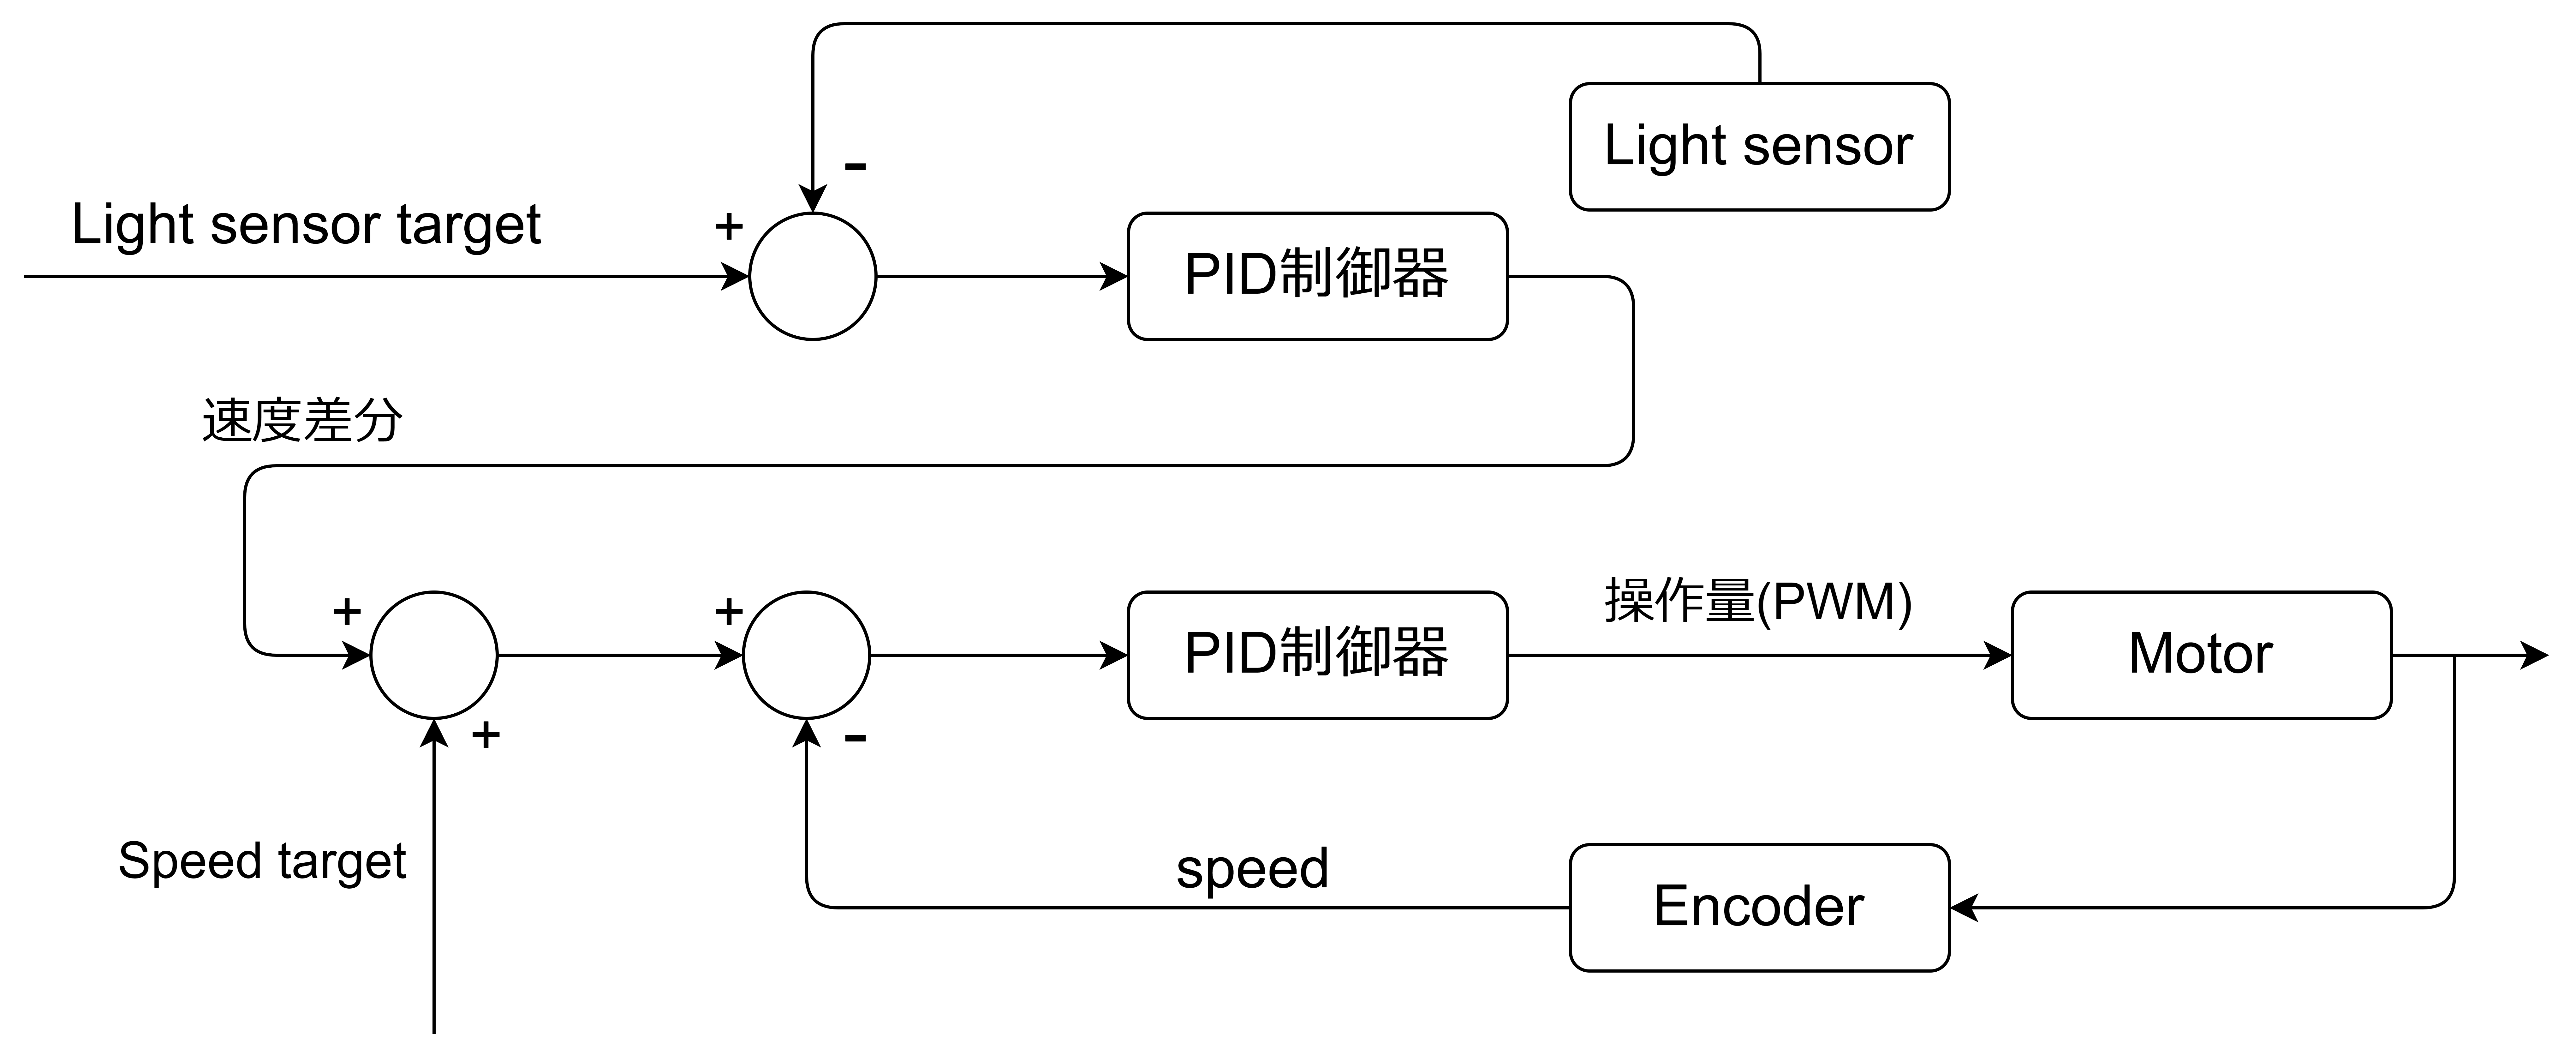
\includegraphics[keepaspectratio, scale=0.5]
       {img/block_line.drawio.png}
  \caption{採用したシステムのブロック線図}
  \label{fig:blockline}
 \end{figure}

PID制御器が2つ直列に接続されていること、および速度のPID制御の前で3つの値の加減算が行われていることが特徴的である。

%制御の具体的な内容は後の\ref{sec:PIDestimate}節から\ref{sec:SensorIntegration}節に記述する。

\section{光センサ値の検出}
\subsection{コース線の中心の推定}
先に述べたように、本機は8つのセンサを積んでいるが、PID制御に回すためには1つのスカラ値に変換する必要がある。センサ値の統合には様々な方法があるが、線が機体の外側に行くほど絶対値の大きい値を返すような単調な関数となっていることが望まれる。
そこで、本機では2つのモータを結んだ線の中心から、コース線の中心と推定される位置の角度をセンサ値として利用する。ここで、コース線が左側にあるとき、負の値を返し、右側にあるときに正の値を返すとする。
位置関係を示すと、図\ref{fig:linepos}のようになる。
\begin{figure}[H]
  \centering
  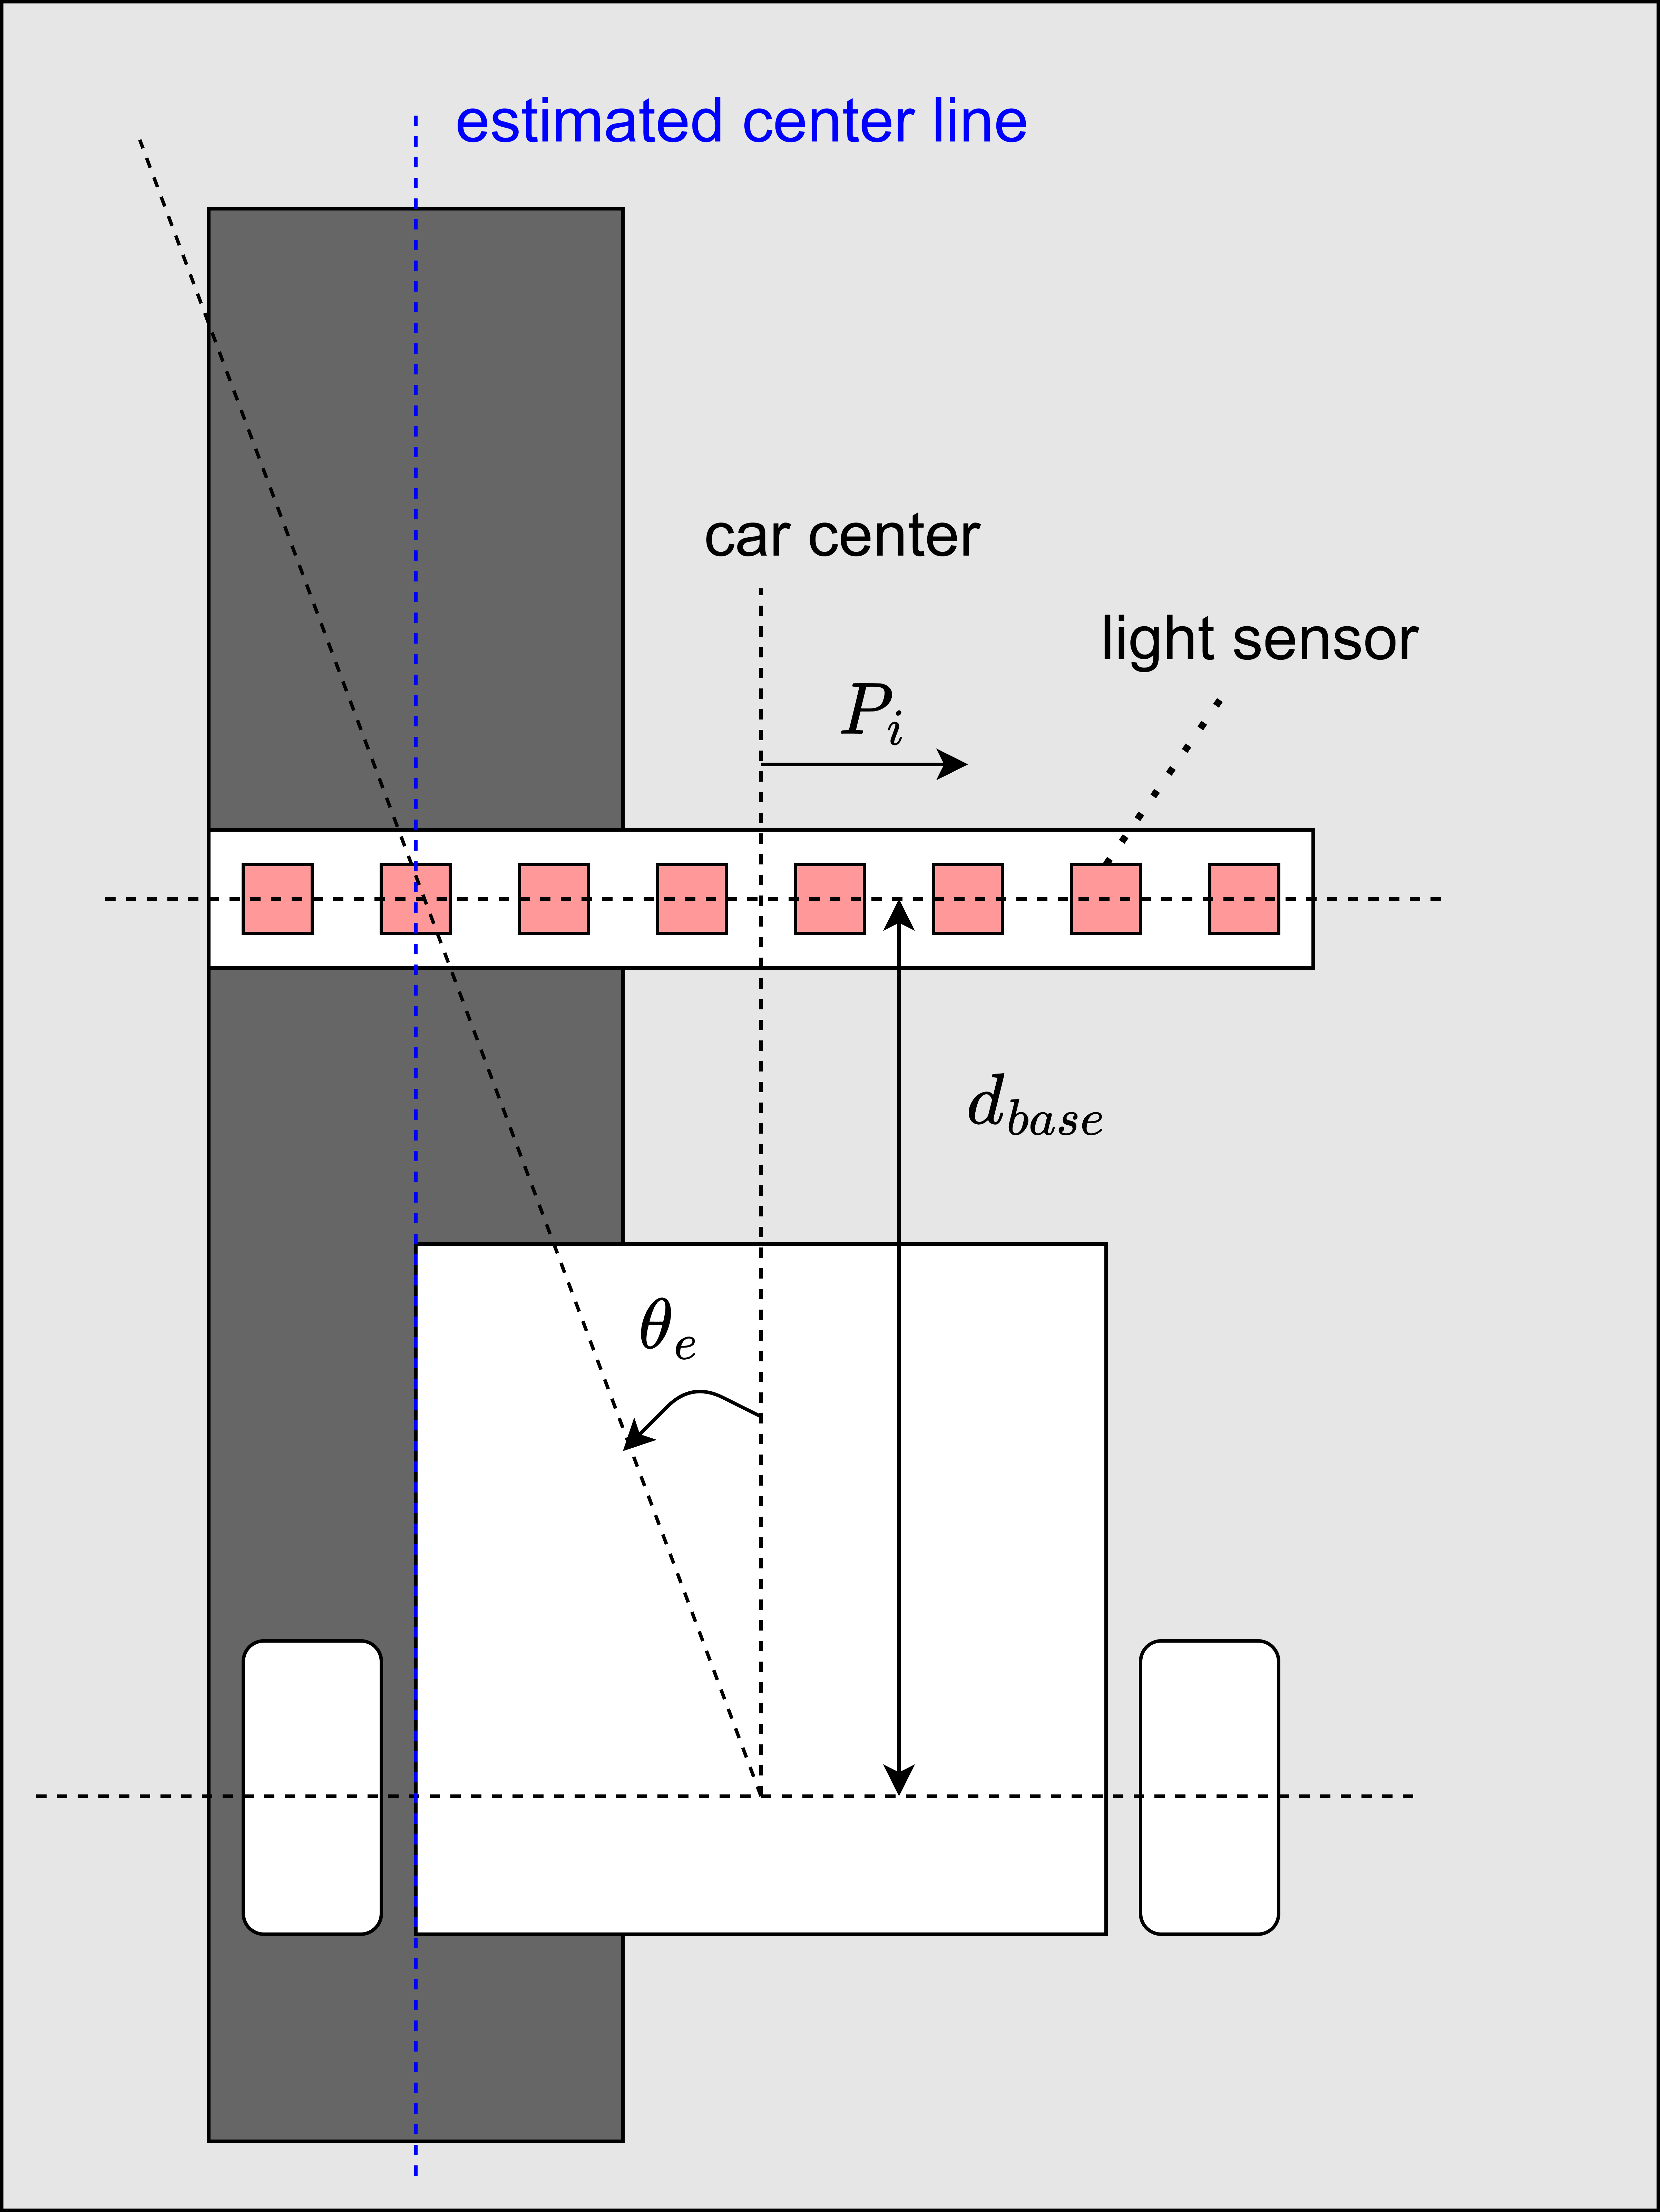
\includegraphics[keepaspectratio, scale=0.5]
       {img/sensor_theta.drawio.png}
  \caption{位置関係}
  \label{fig:linepos}
 \end{figure}


まず、コース線の中心位置を推定する方法を考えよう。
図の左側のセンサから順に0番から7番であるとする。
車体の中心線car\_censorを基準として右側を正、左側を負とする座標系を考えると、
各センサの位置は0番から順に-7, -5, -3, -1, 1, 3, 5, 7 [cm]にある。
つまり、i番目のセンサ位置$P_i$は
\[ 
      P_i = -7 + 2i
\]
である。
次に、センサiがコース線に乗っているか判定する関数を$b[i]$とすれば、

\begin{equation}
  b[i] = 
  \begin{cases}
   1 & (センサiがコース線上にある) \\
   0 & (センサiがコース線上にない)
   \end{cases}
\end{equation}

$b[i]$はセンサの実測値に対してしきい値を付けることで容易に実装することができる。

よって、これらを足し合わせ、"コース線上に乗っている"センサ数Nで割り、平均を取ることでコース線の推定位置$P_e$は

\[ 
  P_e = \frac{1}{N} \sum_{n=0}^7 b[i] P_i
    \]

\subsection{角度の推定}

次に、車軸から見込んだ推定角度$\theta_e$を求めよう。
本機において、車軸とセンサのある位置までの距離$d_{base} = 13 [\mathrm{cm}]$である。また、$\tan \theta_e = \frac{P_e}{d_{base}}$である。
ゆえに、
\[
  \theta_e =  \tan^{-1} \frac{P_e}{d_{base}}
\]
である。

三角関数は計算量が他の演算に対して大きいのでボトルネックとなることがある。その際には、$\tan^{-1}$をテイラー展開して、適当な次数で切ることで冪関数として扱えば良い
\footnote{$\arctan x$のテイラー展開は2次近似まで$x$であるから、大きさの正規化さえ気をつければ$P_e$を直接角度の推定値として扱ってもあまり問題はない。今回は精度を優先した。}。
今回の配置であれば、5次近似程度あれば十分な精度である。
しかし、実際に実験した結果、今回は特にボトルネックにならなかったので、検討はしたものの、特に必要はなかった。

\subsection{読み込みのボトルネック}
以上で8つのセンサを1つのスカラ値に変換することができた。
この処理では8つのセンサを順次読みこむことから、ボトルネックとなり得ることに注意する必要がある。
実は当初設計では採用したマイコンではピンが不足していたのでマルチプレクサを順次切り替えて処理する形式を取っていた。
しかし、実際に試したところ、回路設計の関係なのか、1度切り替えてから電圧が安定するまで110 \mu s 程度要することがわかった\footnote{マルチプレクサ側の問題ではない。モーターのエンコーダも同様にマルチプレクサを使っていたが、3 \mu s程度のディレイで問題なく動作した。}。このディレイは毎回挟むと後述の速度検出のサンプリング周波数が不足するため解消する必要があった。
そのため、本機ではマイコンを2台利用するように設計を変更し、光センサ値の検出に関係する部分をすべて移動した。
遅延への懸念から、光センサ用マイコンから本マイコンへの通信には通信プロトコルを使用せず、適切なレンジにマッピングしたアナログ値(電圧)を出力し、受け取り側で扱いやすい値に再マッピングすることで問題なく利用することができる。
今回は受け取り側で[-10, 10]の範囲に再マッピングした。

\section{速度の検出}
\subsection{エンコーダ}
速度の検出にはモータに付いているエンコーダを活用する。
エンコーダにはホールセンサが付いており、車輪を回転させると、1回転で決まった回数$P$だけデジタルでパルスが送られる。
本機においては$P=11$である。
つまり、信号を$f(t)$とし、モータを定速で回転させたならば$f(t)=1 \; \mathrm{(HIGH)}$となる時間と、$f(t)=0 \; \mathrm{(LOW)}$となる時間を周期的に
繰り返す。
通常モータは正転と逆転を判別するために位相の異なるホールセンサが2つ搭載されている。しかし、今回はモータは逆転しないものとし、1つのエンコーダにのみ着目する。

\subsection{センサ値のサンプリング}
デジタル値が流れている生データから速さを取得するためには、信号の値の変化を捉えてその時間間隔を調べればよい。1つのエンコーダで捉えられる値の変化はHIGH to LOW または LOW to HIGH の2種類である。仮に両方の変化を捉えるとすれば、1回転で$2P$回の変化を捉えることとなる。一般に、より多くの変化を捉えるほうが精度のよい速さが求められるが、サンプリング周波数に注意する必要がある。プログラム中で速度を毎ループ計算せずに非同期で処理する場合、1ループにかかる時間の逆数がサンプリング周波数である。
そして、1ループで1回の変化が起こる状態(毎回のループでHIGH -> LOW -> HIGHと変化している状態)が取得しうる最高速度であり、それ以上の速度は測定できない。しかし、そもそもナイキスト定理を考えれば、この状態はすでにエイリアシングが発生して精度が低下しているから元の信号の周波数は更に低くなければいけない。さらに言えば、ナイキスト定理では2倍のサンプリング周波数があれば良いことになっているが、波形を復元する特別な工夫がないなら10倍以上の周波数を使うべきである。
フーリエ変換を考えて厳密に言えば、デジタル信号は矩形波であるから、無限大の周波数がなければ修復できない。そのため、どのようなサンプリング周波数で計測しても、たまに飛び値が出る。しかし、モータは瞬間的に追従することはできないうえ、次の瞬間には正しい値に戻っていることを考えれば飛び値が出ることは問題にならない。そして、LOW->HIGH->LOWをあたかも1つの波であるかのように捉えてその周波数を考えてみればこの計測法でも比較的正しい速度が計算できることがわかる。こちらで考えても周波数が高すぎるときは、変化の読み落としが発生しているので全く信用にならない。本機ではLOW to HIGHのみを捉えることとする。

ここまでは、非同期で処理する場合を考えた。では同期処理ではどのような問題があるだろうか。
まず、同期処理では毎回の処理でそのときの速度を定める。つまり、毎回速度が確定するまでこの処理のみを実行するので、読み落としは発生せず、エイリアシングの問題等は一切考える必要がない。ここだけ聞くと、同期処理のほうがよく聞こえるかもしれないが、問題はこの処理が終わる(= エンコーダの変化を2点で捉える)まで次の処理に進めないことである。高速走行時には短い時間で変化を捉えられるので大きな問題にはならないかもしれないが、低速時には待ち時間が増えるし、停止時には停止しているかどうかを明確に判別できるだけの最大待ち時間待たなければならなくなる。その時間はモータに依存するが本機においては最低でも20msであった。つまり、1ループに最大20ms、高速走行時でも非同期処理よりは当然遅く、数msの待ち時間が発生する。待ち時間とはつまり制御が入らずに空走する時間である。例えば、50cm/sで走行中に5msの待ち時間があったとすると、空走距離は50cm/s \times 5ms = 0.25cmである。僅かな量に感じるかもしれないが、これだけの空走距離があると急なカーブ等には対応することが困難である。つまり、同期処理で速度を取得すると非常に大きなボトルネックになるので、速度の計算は非同期処理にする必要がある。


\subsection{生データから速さへの変換}
前節でモータ1回転に捉える変化数を決めた。改めて$P$とおく。つまり、本機においては$P=11$である。
次に、値の変化にかかった時間を$\Delta t$ [\mu s] とする。モータのギア比(減速比)をRとする。タイヤの直径を$D$ [cm] とすれば、タイヤ外周部の速度$v$ [cm/s]は次の
ように表される。
\[ v = \frac{\pi D \times 10^6}{R P \Delta t} \]

これは実質的に時間の1変数関数であり、残りは機体に固有の定数であるから、切り分けて前処理に回すことで処理を高速化できることに留意したい。
また、車体が停止しているとき、$\Delta t$は永遠に求まらないため、同期処理と同様に一定時間経過したら速度を0と判定するしきい値時間を用意する必要があることに注意する。

\subsection{非同期処理の実装}
本機はArduino互換ボードを使用しており、ソフトウェアの実装言語はArduino言語である。そのため、Python等高機能言語に実装されているasync/await等の高級な非同期処理インターフェースはない。
そのような状況でシンプルに非同期処理を実装するためには、時間を確認することが有効である。Aruduino言語には、経過ミリ秒を表示するmillis()やマイクロ秒を表示するmicros()が存在するため、それを用いることで素朴な非同期処理を実装することができる。

その他の選択肢としては、今回は採用していないが割り込み処理にする方法が考えられる。
ボード依存であるが、Arduinoは割り込み処理をサポートしている。ホールセンサの信号の変化をトリガとした割り込み処理をすればより
無駄のない速度計測ができる可能性がある。
\subsection{ノイズ対策}
エンコーダでは、ホールセンサの信号をHIGHとLOWで送信する。回転の途中で値の境界付近の状況にあるとき、短い周期で信号が震えることがある。これはスイッチにおけるチャタリングに近い現象であり、同様に対策が必要となる。
本機では、信号値を取得する際に毎ループで続けて3回取得し、すべての信号値が揃わなければ信用できないとして信号を取得し直す、というロジックによりこの問題へ対処した。



\section{モータ制御}


\subsection{センサのPID制御}\label{sec:SensorIntegration}
これまででそれぞれのセンサ値を取ることができた。次にこれをモータの動作に落とし込む必要がある。
改めて、PID制御を時間の式で示せば、
\[
  y = K_p e + K_i \int e \; dt + K_d  \frac{\mathrm{d}e}{\mathrm{d}t}
\]
ただし$e$は目標値から現在値を引いた偏差である。
これはアナログ値であるから、デジタル値による記法に変換する必要がある。これにはいくつかの流儀があるが、今回は最も基本的な方式として、微小時間は無視する、積分要素は面積を取らずに現在差分を単純に足す、微分要素は差分要素に置き換えるという方法を取った。
% TODO: PID式の整合性確認後、デジタル版のPIDを入れる?

今一度PID制御器の結果がどのように使われるか確認しよう。
光センサについてのPIDの結果は曲がる方向に応じてモータの目標速度を変化させる役目をもつ。

%TODO: あとで続きを
%本機体において、センサ値は、メインとは別のマイコンで処理されて送られてくる。送られてきた値は処理しやすいように、[-10, 10]の範囲にマッピングするものとする。
図\ref{fig:blockline}にブロック線図を示してあるから、あと必要なことはそのまま実装して、パラメータの調節を行うことのみ(これが一番大変かもしれない!)である。

\subsection{光センサにおけるPID調整前のパラメータ推定}\label{sec:PIDestimate}
PID制御のパラメータ調節は地道な作業であるが、論理的に考えられる部分については、ある程度あたりをつけてから始めると楽である。
特に、PID制御の調節はP制御から始め、$K_p$の大きさによって他の値のレンジの決定されるので、$K_p$の正当性が最も重要である。
ここでは、光センサのP制御値について考察を行うことでパラメータにあたりをつけてみよう。

ライントレースを行ううえで一番走行が難しいのは急カーブである。逆にいえば、急カーブを走行してもコースアウトせずに即座に車体の安定を取り戻せる状態なら他の場所は問題にならない。では$K_p$をいったいどのくらいの大きさにすれば最も急なカーブを曲がり切れるだろうか?

最も急なカーブの曲率半径を$r$[cm]とする。車体の中心線からタイヤの中心までの距離を$d$[cm]とする。与えた走行速度目標を$v_t$[cm/s]とする。ここで、走行速度目標とはカーブに差し掛かって光センサ値による補正がかかった値ではなく、光センサ値によらない(つまり、直進中の値とも言える)である。
ある瞬間、走行体は角速度$\dot{\theta}$[rad/s]で円運動をしているとしよう。このとき、機体の制御により、外側の車輪の目標速度は$v_t + \Delta v$、内側の車輪の速度は$v_t - \Delta v$に変更される。ただし、$\Delta v $は$K_p$に依存する値である。このとき、速度に関する次の2つの式が成り立つ。

\begin{align}
  v_t + \Delta v &= (r+d)\dot{\theta}\\
  v_t - \Delta v &= (r-d)\dot{\theta}
\end{align}
ここから$\dot{\theta}$を削除することにより、
\begin{align}
  \frac{v_t+ \Delta v}{v_t-\Delta v} &= \frac{r+d}{r-d}\\
                                    &= k
\end{align}
とおくと、$k$は$r$と$d$によって決まるからコースと車体のプラットフォームが変わらない限り定数である。
このkを用いると、
\[
  \Delta v = \frac{k-1}{k+1}v_t
\]
と表される。つまり、光センサのPID制御全体で$\Delta v$ より大きい速度の変化分を出せないと曲がりきれないことが実験しなくてもわかる。

本機体について考えてみよう。
本機体において、$d=7.5$[cm]
速度$v_t =100$[cm/s]で、曲率半径$r=10$[cm]の円を曲がるとする。このとき、$k = 7$であるから、
$\Delta v = \frac{6}{8}v_t = \frac{3}{4}\times 100 = 75$である。
いま、光センサ値が[-10, 10]の範囲でマッピングされている。現在の光センサの値を$l$とする。
光センサの目標値は中心である0とすれば$e=l$。
P制御しか行わない状態を仮定すると、$\Delta v = K_p |l| > 75$となる。
光センサが最大値のときにぎりぎり曲がりきれると仮定すると、$l=\pm 10$で、$K_p > 7.5$となる。
実際にはもっと余裕を持ちたいのでより大きな値となると推定される。
たとえば、$l=8$で曲がりきりたいとすると、$K_p > 9.38$程度となる。
これとD制御を組み合わせることで、急なカーブでもより安定して走行することができる。

実際に採用した値が$K_p=10.0, K_d = 12.5, K_i = 0.0002$であることを考えるとこの考察は非常に有益であることがわかる。



\subsection{アドホックな調整}
%ダンパーとsk
ここまでで、カーブを含めたほとんどの場合において安定した走行をするための議論は完了した。
しかし、まだ特殊な場合で安定しない可能性が残されている。本節ではそのような特定の状況に対応するアドホックな処理について議論する。

安定しない可能性があるのは速度0からの立ち上がりの状況である。
理由は2つある。

1つ目は、目標速度を大きくすればするほど、初めのP制御が強く効くからである。
理想的状況であれば、速やかに目標速度に到達するため問題ない。しかし、左右のモータの回りやすさに差がある場合、初めの制御量が大きく入ると左右差が大きく出やすく、場合によっては修正する間もなくコースアウトしてしまう。

これに対応するためには立ち上がりの偏差に制限をかければよい。つまり、両輪が低速時に限り、現在速度から逆算したターゲット速度を与えることで実現される。これは、数式モデルとしては異なるが、一次遅れ要素に似た性質をもつ。
つまり、以下のようにすればよい。
\begin{verbatim}
  DelayAccelerationSpeed(targetSpeed, maxError, leftCurrentSpeed, RightCurrentSpeed)
    if leftCurrentSpeed < threshold and rightCurrentSpeed < threshold
      newTargetL = min(leftCurrentSpeed + maxError, targetSpeed)
      newTargetR = min(RightCurrentSpeed + maxError, targetSpeed)
      return newTargetL, newTargetR
    else
      return TargetSpeed, TargetSpeed
\end{verbatim}
副次的効果として、偏差の最大値が部分的ではあるが制限されることになるため、モータ側のPID制御の$K_p$をより大きくしても問題が起こりにくくなる。すべての場合で偏差の最大値を制限すれば偏差がmaxError以下であることが保証されるのでそれを念頭に置いた設計ができるが、急カーブを曲がりにくくなるという難点があるため推奨しない。

安定しないもう1つの理由は、センサのPID制御値の速度依存性である。
\ref{sec:PIDestimate}節で速度に応じて与えるべきセンサの$K_p$が変化することを述べた。
もちろん$K_p$は目標速度に合わせて作られているから、立ち上がりの速度ではいささか強く効きすぎる。
そして、先に述べたように、モータには個体差があるから同じように操作量を与えてもまっすぐに進み出すわけではない。
その結果、低速でラインを跨ごうとし、一方の車輪が完全に止まろうとする、逆向きに曲がろうとしてもう一方の車輪が完全に止まろうとする、という動作を繰り返して、振動的な挙動をしながら加速する。このような挙動ではスムーズな立ち上がりとは言えないから、対処したほうがよい。

これに対応する解決策も単純であり、両輪が低速であるときにはセンサのPIDの係数を書き換えれば良い。
もちろんなめらかに変化させることもできるが、低速用の係数を用意して、書き換えるか、書き換えないかという2段階があれば十分であると思われる。
本機の場合は、50cm/sにチューニングしたPID値を用意して二段階にしておけば十分安定した走り出しとなった。

\subsection{Xbeeとの通信}
低速で走行実験を行う場合、万が一コースアウトしても手で止めに行けば問題にならない。
しかし、100cm/sといった高速で走行する場合、手で止めると機体にダメージが入ったり、手で止める前に壁に衝突する危険性がある。
走行会の前に事故によって機体が破損するといった事態は絶対に避けなければならない。
これを避けるため、遠隔で発進と緊急停止を行うことができる機能があるとよい。
やり方は様々あると考えられるが、本機ではXbeeを搭載して遠隔シリアル通信による発進と停止の機能を実装した。


\section{ソースコード}
長くなるので、GitHubのリポジトリに上げてある。
リンクは\url{https://github.com/RiceCake1/LineFollow/tree/main}

この節では、実装を関数別に簡単に解説する。
なお、Arduinoではデフォルトでsetup関数とloop関数が必要である。
setup関数は起動時に1度だけ呼ばれる関数であり、ピンの設定や、初期化等を書く場所である。
loop関数はsetup関数のあとに常に呼ばれる関数であり、メインループとなっている。
\subsection{光センサ関係}
%TODO: 書いていこう!

\subsection{エンコーダ関係}

\subsection{モータの制御関係}

\subsection{その他}

\chapter{評価}

\section{ループ速度}


\section{実測記録}


\section{感想}




\appendix

\chapter{応用的な電気回路解析}
\section{4端子回路}

\section{ひずみ波交流の解析}

\section{三相交流}

\section{分布定数回路}


\chapter{設計の変遷}
本付録では、最終成果物に至るまでの設計の変遷を示す。
\section{初号機}


\section{センサ値の統合}



\chapter{インシデント、問題解決集}





\end{document}